\documentclass[12pt,a4paper,oneside]{book}
\usepackage{lmodern}
\usepackage{xcolor}

\definecolor{vert1}{rgb}{0.0,0.3.9,0.0}
\definecolor{bleu}{rgb}{0,0,0.5}
\definecolor{bleu3}{rgb}{1,0.2,0.2}

\usepackage[utf8]{inputenc}
\usepackage[T1]{fontenc}
\usepackage[francais]{babel}
\usepackage[top=1.7cm, bottom=1.7cm, left=1.5cm, right=1.5cm]{geometry}
\usepackage{pdfpages}
\usepackage{listingsutf8}
\usepackage{fancyhdr}
\usepackage{multido}
\usepackage{amssymb}
\usepackage{tikz}
\usepackage{ifthen}
\usepackage{wrapfig}
\usepackage{makeidx}
\usepackage[urlbordercolor={1 1 1}, linkbordercolor={1 1 1}, linkcolor=vert1, urlcolor=bleu, colorlinks=true]{hyperref}
\usepackage{float}

\newcommand{\footCentre}{}
\newcommand{\premierDestinataire}{Monsieur Thierry Millan}
\newcommand{\rolePremierDestinataire}{Client}

\newcommand{\secondDestinaire}{Madame Caroline Kross}
\newcommand{\roleSecondDestinaire}{Tutrice}

\newcommand{\troisiemeDestinaire}{}
\newcommand{\roleTroisiemeDestinaire}{}

\newcommand{\quatriemeDestinaire}{}
\newcommand{\roleQuatriemeDestinaire}{}

\newcommand{\cinquiemeDestinaire}{}
\newcommand{\roleCinquiereDestinaire}{}

\newcommand{\titreDocument}{Installation et exploitation}



\date{\today}

\chead{\headCentre}
\rhead{\headDroite}
\lhead{\headGauche}
\makeindex
\lfoot{Université Paul Sabatier Toulouse III}
\rfoot{--~\thepage~--}
\cfoot{\footCentre}
\makeglossary
\makeatletter
\def\clap#1{\hbox to 0pt{\hss #1\hss}}%
\def\ligne#1{%
\hbox to \hsize{%
\vbox{\centering #1}}}%
\def\haut#1#2#3{%
\hbox to \hsize{%
\rlap{\vtop{\raggedright #1}}%
\hss
\clap{\vtop{\centering #2}}%
\hss
\llap{\vtop{\raggedleft #3}}}}%
\def\bas#1#2#3{%
\hbox to \hsize{%
\rlap{\vbox{\raggedright #1}}%
\hss \clap{\vbox{\centering #2}}%
\hss
\llap{\vbox{\raggedleft #3}}}}%
\def\maketitle{%
\thispagestyle{empty}\vbox to \vsize{%
\haut{}{\@blurb}{}
\begin{flushleft}
	\vspace{1cm}
	Antoine de \bsc{Roquemaurel}\\ 
	Mathieu \bsc{Soum}\\
	Geoffroy \bsc{Subias}\\
	Marie-Ly \bsc{Tang}\\
	\textit{Groupe B}\\
\end{flushleft}
\begin{flushright}
	\vspace{-3cm}
	\ifthenelse{\equal{\premierDestinataire}{}}{
	}
	{
		Pour \premierDestinataire(\rolePremierDestinataire)\\
	}
	\ifthenelse{\equal{\secondDestinaire}{}}{
	}
	{
		Pour \secondDestinaire(\roleSecondDestinaire)\\
	}
	\ifthenelse{\equal{\troisiemeDestinaire}{}}{
	}
	{
		Pour \troisiemeDestinaire(\roleTroisiemeDestinaire)\\
	}
	\ifthenelse{\equal{\quatriemeDestinaire}{}}{
	}
	{
		Pour \quatriemeDestinaire(\roleQuatriemeDestinaire)\\
	}
	\ifthenelse{\equal{\cinquiemeDestinaire}{}}{
	}
	{
		Pour \cinquiemeDestinaire(\roleCinquiereDestinaire)\\
	}
\end{flushright}
\vfill
\vspace{1cm}
\begin{flushleft}
\usefont{OT1}{ptm}{m}{n}
\huge \@title
\end{flushleft}
\par
\hrule height 4pt
\par
\begin{flushright}
\usefont{OT1}{phv}{m}{n}
\Large \@author
\par
\end{flushright}
\vspace{1cm}
\vfill
\vfill
\bas{}{\@location, le \@date}{}
}%
\cleardoublepage
}
\def\date#1{\def\@date{#1}}
\def\author#1{\def\@author{#1}}
\def\title#1{\def\@title{#1}}
\def\location#1{\def\@location{#1}}
\def\blurb#1{\def\@blurb{#1}}
\date{\today}
\author{}
\title{}
\location{Amiens}\blurb{}
\makeatother
\title{\titreDocument}
\author{Bibliothèque d'objets graphiques UML}

\location{Toulouse}
\blurb{%
Université Paul Sabatier -- Toulouse III\\
IUT A - Toulouse Rangueil\\
\textbf{Projet tuteuré}\\[1em]
}%



\pagestyle{fancy}

\definecolor{gris1}{gray}{0.40}
\definecolor{gris2}{gray}{0.55}
\definecolor{gris3}{gray}{0.65}
\definecolor{gris4}{gray}{0.50}
\definecolor{vert}{rgb}{0,0.4,0}
\definecolor{bleu1}{rgb}{0,0,0.8}
\definecolor{bleu2}{rgb}{0,0.2,0.6}
\definecolor{bleu3}{rgb}{0,0.2,0.2}


\lstdefinelanguage{algo}{%
   morekeywords={%
    %%% couleur 1
		importer, programme, glossaire, fonction, procedure, constante, type, 
	%%% IMPORT & Co.
		si, sinon, alors, fin, tantque, debut, faire, lorsque, fin lorsque, 
		declenche, declencher, enregistrement, tableau, retourne, retourner, =, 
		/=, <, >, traite,exception, 
	%%% types 
		Entier, Reel, Booleen, Caractere, Réél, Booléen, Caractère,
	%%% types 
		entree, maj, sortie,entrée,
	%%% types 
		et, ou, non,
	},
  sensitive=true,
  morecomment=[l]{--},
  morestring=[b]',
}

\lstset{language=algo,
    %%% BOUCLE, TEST & Co.
      emph={importer, programme, glossaire, fonction, procedure, constante, type},
      emphstyle=\color{bleu2},
    %%% IMPORT & Co.  
	emph={[2]
		si, sinon, alors, fin , tantque, debut, faire, lorsque, fin lorsque, 
		declencher, retourner, et, ou, non,enregistrement, retourner, retourne, 
		tableau, /=, <, =, >, traite,exception
	},
      emphstyle=[2]\color{bleu1},
    %%% FONCTIONS NUMERIQUES
      emph={[3]Entier, Reel, Booleen, Caractere, Booléen, Réél, Caractère},
      emphstyle=[3]\color{gris1},
    %%% FONCTIONS NUMERIQUES
      emph={[4]entree, maj, sortie, entrée},	
      emphstyle=[4]\color{gris1},
}
\lstdefinelanguage{wl}{%
   morekeywords={%
    %%% couleur 1
		importer, programme, glossaire, fonction, procedure, constante, type, 
	%%% IMPORT & Co.
		si, sinon, alors, fin, TANTQUE, tantque, FIN, PROCEDURE, debut, faire, lorsque, 
		fin lorsque, declenche, declencher, enregistrement, tableau, retourne, retourner, =, 
		/=, <, >, traite,exception, 
	%%% types 
		Entier, Reel, Booleen, Caractere, Réél, Booléen, Caractère,
	%%% types 
		entree, maj, sortie,entrée,
	%%% types 
		et, ou, non,
	},
  sensitive=true,
  morecomment=[l]{//},
  morestring=[b]',
}

\lstset{language=wl,
    %%% BOUCLE, TEST & Co.
      emph={importer, programme, glossaire, fonction, procedure, constante, type},
      emphstyle=\color{bleu2},
    %%% IMPORT & Co.  
	emph={[2]
		si, sinon, alors, fin , tantque, debut, faire, lorsque, fin lorsque, 
		declencher, retourner, et, ou, non,enregistrement, retourner, retourne, 
		tableau, /=, <, =, >, traite,exception
	},
      emphstyle=[2]\color{bleu1},
    %%% FONCTIONS NUMERIQUES
      emph={[3]Entier, Reel, Booleen, Caractere, Booléen, Réél, Caractère},
      emphstyle=[3]\color{gris1},
    %%% FONCTIONS NUMERIQUES
      emph={[4]entree, maj, sortie, entrée},	
      emphstyle=[4]\color{gris1},
}
\lstdefinelanguage{css}{%
   morekeywords={%
    %%% couleur 1
		background, image, repeat, position, index, color, border, font, 
		size, url, family, style, variant, weight, letter, spacing, line, 
		height, text, decoration, align, indent, transform, shadow, 
		background, image, repeat, position, index, color, border, font, 
		size, url, family, style, variant, weight, letter, spacing, line, 
		height, text, decoration, align, indent, transform, shadow, 
		vertical, align, white, space, word, spacing,attachment, width, 
		max, min, margin, padding, clip, direction, display, overflow,
		visibility, clear, float, top, right, bottom, left, list, type, 
		collapse, side, empty, cells, table, layout, cursor, marks, page, break,
		before, after, inside, orphans, windows, azimuth, after, before, cue, 
		elevation, pause, play, during, pitch, range, richness, spek, header, 
		numeral, punctuation, rate, stress, voice, volume,
	%%% types 
		left, right, bottom, top, none, center, solid, black, blue, red, green,
	},
  sensitive=true,
  sensitive=true,
  morecomment=[s]{/*}{*/},
  morestring=[b]',
}
\lstset{language=css,
    %%% BOUCLE, TEST & Co.
      emph={
		background, image, repeat, position, index, color, border, font, 
		size, url, family, style, variant, weight, letter, spacing, line, 
		height, text, decoration, align, indent, transform, shadow, 
		background, image, repeat, position, index, color, border, font, 
		size, url, family, style, variant, weight, letter, spacing, line, 
		height, text, decoration, align, indent, transform, shadow, 
		vertical, align, white, space, word, spacing,attachment, width, 
		max, min, margin, padding, clip, direction, display, overflow,
		visibility, clear, float, top, right, bottom, left, list, type, 
		collapse, side, empty, cells, table, layout, cursor, marks, page, break,
		before, after, inside, orphans, windows, azimuth, after, before, cue, 
		elevation, pause, play, during, pitch, range, richness, spek, header, 
		numeral, punctuation, rate, stress, voice, volume,
	  },
      emphstyle=\color{bleu2},
    %%% FONCTIONS NUMERIQUES
      emph={[3]
		left, right, bottom, top,none, solid, black, blue, green,
		  },
      emphstyle=[3]\color{bleu3},
    %%% FONCTIONS NUMERIQUES
}
\lstdefinelanguage{SQL}{%
   morekeywords={%
    %%% couleur 1
	INSERT, if, end, begin,UPDATE, DELETE, SET, WHERE, 
	CREATE, OR, REPLACE, AND, FROM, SELECT, VIEW, TRIGGER, AS, GROUP,
	BY, ORDER, after, for, each, then, else, of, on
	},
  sensitive=true,
  morecomment=[l]{--},
  morestring=[b]',
}

\lstset{language=SQL,
    %%% BOUCLE, TEST & Co.
      emph={INSERT, UPDATE, DELETE, WHERE, SET, GROUP, BY, ORDER},
      emphstyle=\color{bleu2},
    %%% IMPORT & Co.  
	emph={[2]
		if, end, begin, then, for, each, else, after, of, on
	},
      emphstyle=[2]\color{bleu1},
    %%% FONCTIONS NUMERIQUES
      emph={[3]Entier, Reel, Booleen, Caractere, Booléen, Réél, Caractère},
      emphstyle=[3]\color{gris1},
    %%% FONCTIONS NUMERIQUES
      emph={[4]entree, maj, sortie, entrée},	
      emphstyle=[4]\color{gris1},
}
\lstset{ % general style for listings 
   numbers=left 
   , literate={é}{{\'e}}1 {è}{{\`e}}1 {à}{{\`a}}1 {ê}{{\^e}}1 {É}{{\'E}}1 {ô}{{\^o}}1 {€}{{\euro}}1{°}{{$^{\circ}$}}1 {ç}{ {c}}1 {î}{{\^i}}1
	, extendedchars=\true
   , tabsize=2 
   , frame=single 
   , breaklines=true 
   , basicstyle=\ttfamily 
   , numberstyle=\tiny\ttfamily 
   , framexleftmargin=0mm 
   , xleftmargin=0mm 
   , captionpos=b 
	, keywordstyle=\color{bleu2}
	, commentstyle=\color{vert}
	, showstringspaces=false
	, extendedchars=true
	, mathescape=true
} 

\begin{document}
	\maketitle
	\setcounter{tocdepth}{1}
	\setcounter{secnumdepth}{3}
	\frontmatter
	\chapter*{Avant-propos}
\nouveauChapitre
\addcontentsline{toc}{chapter}{Avant-propos}
\section*{Présentation du projet}
\addcontentsline{toc}{section}{Présentation du projet}
	LibUML est une 
	\glo{bibliothèque}{Bibliothèque}{Composant programmé dans un langage donné fournissant des méthodes permettant d'effectuer des tâches voulut} 
	d'objets graphiques représentant les différents éléments de modélisation de la norme 
	\glo{UML}{UML}{(Unified Modeling Language) Langage de modélisation graphique à base de pictogramme.  Il est apparu dans le monde du génie logiciel dans le cadre de la conception orientée objet. Ce langage est composé de différents diagrammes, allant du développement à la simple analyse des besoins.} 
	2\footnote{Unified Modelling Language}.
	Celle-ci à été développé dans le cadre des projets tuteurés à l'IUT\footnote{Institut Universitaire de Technologies} 'A' de Toulouse. 
	Nous l'avons développée en \glo{Java}{Java}{Langage de programmation orienté objet moderne, il compile le programme pour ensuite l'exécuter sur une machine Java, ainsi le programme une fois compilé peut être exécuté sur différentes plateformes (Windows, Linux, Mac OS X, \ldots).} 
	et conçut comme une bibliothèque pouvant être utilisée dans des programmes Java comme composant. 
	Vous pouvez vous en servir pour développer un outil complet de modélisation UML par exemple.
	\paragraph{}	
	Cette bibliothèque permet de faire différentes choses dans le cadre de la conception UML, une fois la
	que vous aurez compris le fonctionnement de libUML vous pourrez:
	\begin{itemize}
		\item Créer des éléments de modélisation 
			\begin{itemize}
				\item Acteur actif ou passif
				\item Traitement
				\item Cas d'utilisation
				\item Classe
			\end{itemize}
		\item Relier ses composants via différents types de flèches
			\begin{itemize}
				\item Agrégation
				\item Composition
				\item Association binavigable ou mononavigable
				\item Messages synchrones ou asynchrones
				\item Généralisation
			\end{itemize}
		\item Supprimer des éléments et flèches
		\item Modifier le contenu des éléments et flèches
		\item Redimensionner les éléments de modélisation
	\end{itemize}
	\paragraph{}
Ce document à pour but de vous présenter le fonctionnement de la bibliothèque UML et de son démonstrateur. 

\section*{Présentation du groupe}
\addcontentsline{toc}{section}{Présentation du groupe}
	Notre groupe projet est composé de quatre étudiants de deuxième année de DUT Informatique à l'IUT 'A' de Toulouse, voici la composition de l'équipe: 
	\begin{itemize}
		\item Antoine de \bsc{Roquemaurel} 
		\item Mathieu \bsc{Soum} 
		\item Geoffroy \bsc{Subias}
		\item Marie-Ly \bsc{Tang} 
	\end{itemize}
	\section*{Téléchargements}
\addcontentsline{toc}{section}{Téléchargements}
	Nous vous avons envoyé deux archives zip par email, une contenant le projet Netbeans de la bibliothèque et du démonstrateur et une contenant la bibliothèque.
	\subsubsection*{Bibliothèque et démonstrateur}
	La première archive est donc un projet netbeans, cette archive contient notre bibliothèque et ses tests associés, le démonstrauteur mais
	également la bibliothèque \texttt{JGraphx} qui est indispensable au bon fonctionnement de notre bibliothèque. Nous ne garantissons le bon fonctionnement 
	de la bibliothèque qu'avec la version de \texttt{JGraphx} 1.8, celle-ci n'ayant pas été testé avec des versions différentes.

	Le projet netbeans de notre bibliothèque est également disponible en ligne, si vous souhaitez la télécharger de nouveau, elle est donc disponible à l'adresse suivante: \\
	$\rhd$ \url{http://telechargements.joohoo.fr/libUML/libUML-netbeans.zip}\\
	$\rhd$ \url{http://telechargements.joohoo.fr/libUML/JGraphX-1.8.jar}\\
	
	\subsubsection*{Documentation}
	Toute la documentation du projet est sous format \bsc{HTML}\footnote{HyperText Markup Language}, celle-ci ayant été générée grâce à Javadoc.

	Si dans ce manuel nous parlons d'une méthode et que vous n'en comprenez pas l'intéret, vous pouvez aller la chercher dans la documentation, pour chaque classe,
	le fonctionnement global de la classe est expliquée, l'utilité de chaque attribut, de chaque méthode, et ce que vous devez mettre dans les différents paramètres 
	des méthodes.  
	\paragraph{}
	Nous vous avons remis un .zip par email contenant quatre dossiers de documentation:
	\begin{itemize}
		\item La documentation privée de la \textit{bibliothèque} (Toutes les méthodes et tous les attributs)
		\item La documentation publique de la \textit{bibliothèque} (Seuls les méthodes et attributs publiques ou protégées)
		\item La documentation privée du \textit{démonstrateur} (toutes les méthodes du démonstrateur) 
		\item La documentation des \textit{tests unitaires} (Toutes les méthodes de tests)
	\end{itemize}
	\paragraph{}
	Celle ci est également disponible en ligne aux adresses suivantes: \\
	$\rhd$ \url{http://documentation.joohoo.fr/libUML/bibliothequePrivee/index.html}\\
	$\rhd$ \url{http://documentation.joohoo.fr/libUML/bibliothequePublique/index.html}\\
	$\rhd$ \url{http://documentation.joohoo.fr/libUML/demonstrateurPrivee/index.html}\\\label{docDemonstrateur}
	$\rhd$ \url{http://documentation.joohoo.fr/libUML/testsUnitaires/index.html}\\
	\paragraph{}
	Vous pouvez également accéder à la documentation de \texttt{JGraphX}, cela peut vous être utile dans certains cas.\\
	$\rhd$ \url{http://documentation.joohoo.fr/JGraphX/index.html}\\ 


	\newpage
\section*{Fonctionnement du document}
\addcontentsline{toc}{section}{Fonctionnement du document}
Ce document est un document expliquant notre approche pour développer une bibliothèque d'objets graphiques UML.\\

Dans ce dossier, vous pourrez repérer diverses notations, cette partie a pour but de vous expliquer les notations afin
que vous puissiez lire en toute sérénité.
\subsubsection*{Le glossaire}
Un mot dans le glossaire a une police particulière, vous pourrez savoir qu'un mot est dans le glossaire lorsque vous repérerez un mot avec la police suivante: 
\policeGlossaire{leMotDansLeGlossiare}. Si vous voyez cette police, vous pouvez donc vous référez à l'annexe \ref{glossaire} page \pageref{glossaire}.
\subsubsection*{Les noms de méthode, d'attribut ou de classe}
Les mots se référant à un nom présent dans du code ont une police particulière, une police type ``machine à écrire'', si vous voyez la police suivante, c'est que c'est un nom 
de méthode, d'attribut ou de classe: \texttt{uneFonction}.
\subsubsection*{Les noms de paquetage}
Les noms de paquetage utiliseront une police particulière, afin que l'on puisse les différencier d'une classe ou d'une méthode, vous les trouverez 
comme suit : \policePackage{unPaquetage}.
\subsubsection*{Les notes de bas de page}
Nous utilisons régulièrement des notes de bas de pages, pour donner un acronyme, pour expliquer plus en détail une notion, ces notes de bas de pages sont un numéro
en exposant, vous trouverez la note correspondante en bas de la page courante, comme ceci\footnote{Ceci est une note de bas de page}.
\subsubsection*{Les liens hypertextes}
Dans le document, nous pouvons faire référence à un lien d'un site web, tous les liens seront donc symbolisés par une petite puce, et une police particulière comme ceci:\\
	$\rhd$ \url{http://monLien.fr/index.html}\\
	Une liste de tous les liens présents dans le document est accessible en annexe \ref{listeLiens} page \pageref{listeLiens}.


	\tableofcontents
	\nouveauChapitre
	\newpage
	\mainmatter
	\chapter{Le démonstrateur}
	\section{Interface Homme Machine}
	\nouveauChapitre
	Nous avons développé un démonstrateur afin que vous puissiez comprendre comment fonctionne la bibliothèque, et pour montrer ses possibilités.
	Ainsi, tout ce qu'il est possible de faire avec la bibliothèque sera présent dans le démonstrateur.

	Dans cette partie nous allons passer brièvement ses fonctionnalités, cependant, pour une meilleure
	compréhension, nous avons commenté le code du démonstrateur pour qu'il soit le plus simple possible et pour que vous ayez le moins 
	besoin de vous référez à ce document. La documentation est également disponible au format \glo{javadoc}{Javadoc}{Javadoc est un système de documentation automatique 
	pour Java, cette documentation est générée au format HTML.
	Il analyse les commentaires introduits dans le programme, ceux-ci étant un peu particuliers.} comme signalé en Avant-propos page \pageref{docDemonstrateur}.
	\paragraph{}	
	Le démonstrateur est volontairement simple, il n'a pas pour but d'être lourd, mais uniquement de montrer les possibilités de la bibliothèque. 
	Il est disposé en trois parties:
	\begin{enumerate}
		\item En haut, la barre d'outils, permettant de sélectionner l'élément graphique souhaité
		\item Au centre, ce que nous appelons le graphe, c'est ici qu'apparaîtrons les diagrammes UML
		\item À droite, un panneau contenant éventuellement un tableau avec les informations de la classe sélectionnée, mais aussi le type de diagramme choisit
	\end{enumerate}
	\begin{figure}[H]
		\centering
		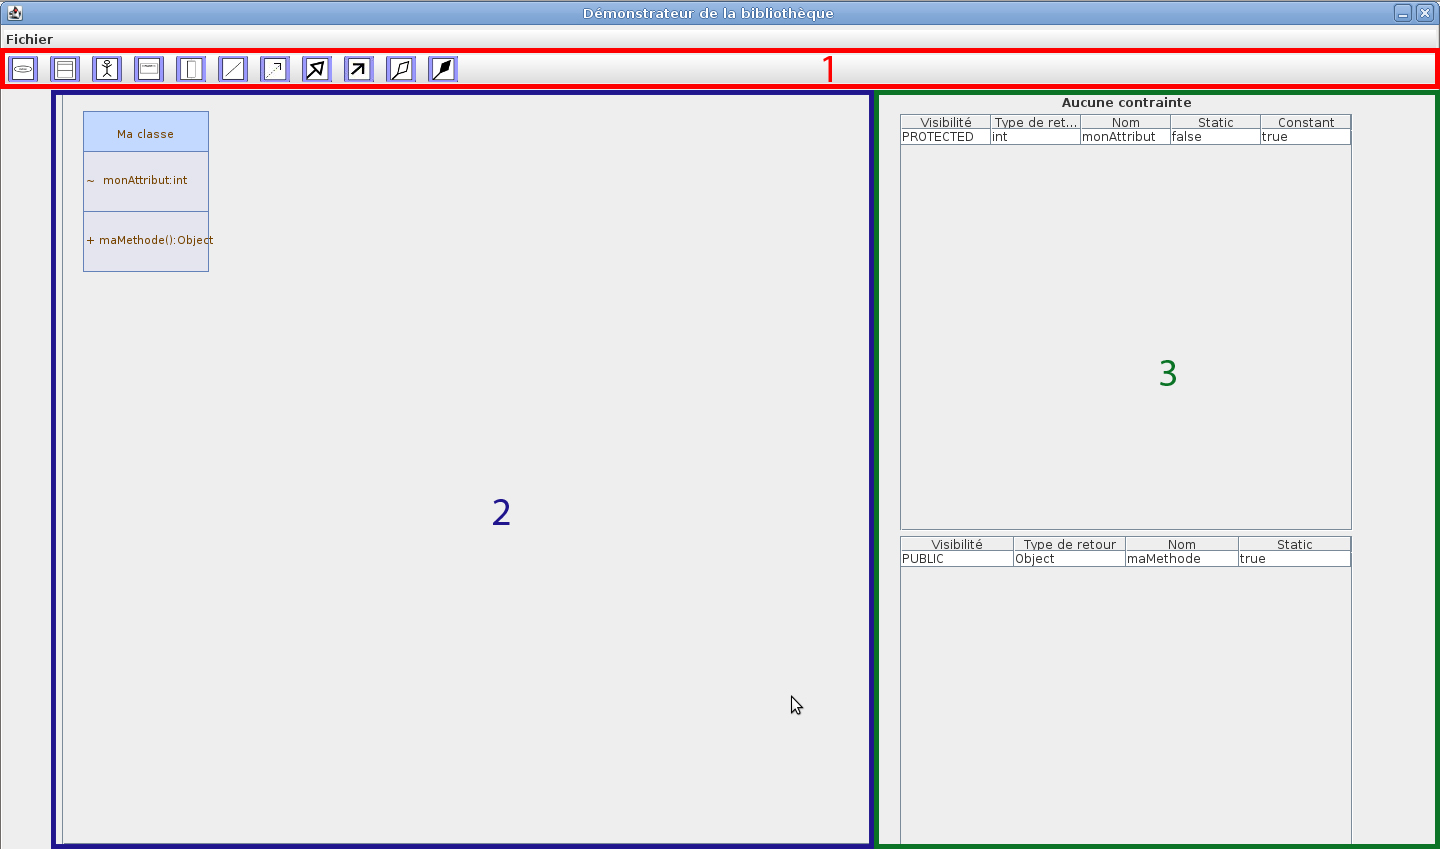
\includegraphics[width=15cm]{screen1.jpg}
		\caption{Les différentes parties du démonstrateur}
	\end{figure}
	Au démarrage du démonstrateur, il faut choisir le type de contrainte souhaitée, cela aura pour effet d'interdire l'ajout de certains éléments.
	\subsection{La barre d'outils}
	La barre d'outils contient tous les éléments graphiques que notre bibliothèque permet d'introduire.
	\subsubsection{Élément de modélisation}
	Il est actuellement possible de faire les éléments de modélisation suivants:
	\begin{itemize}
		\item Acteur actif
		\item Acteur passif
		\item Traitement
		\item Cas d'utilisation
		\item Classe
		\item Interface
	\end{itemize}
	Le clic sur un bouton positionnera un élément de modélisation dans le graphe.

	\subsubsection{Liens}
	La deuxième partie de la barre d'outils contient tous les liens qu'il est possible de faire.
	\begin{itemize}
		\item Association
		\item Dépendance fonctionnelle
		\item Généralisation
		\item Agrégation
		\item Composition
	\end{itemize}
		Pour relier deux éléments, vous devez cliquer sur la flèche voulue, puis cliquer sur les deux éléments à relier. 
	Le clic sur les deux éléments aura pour effet de créer un lien.\\
	Attention, pour les traitements et les classes, la sélection de l'élément se fait par le haut de l'élément.
	\subsection{Le graphe}
	Le graphe contient tous les éléments graphiques, l'affichage d'un élément se fera donc dans le graphe. 
	C'est également dans le graphe que s'affiche le menu contextuel permettant d'interagir avec les éléments.

	Le graphe est également important dans la programmation comme nous le verrons section \ref{mxGraph} page \pageref{mxGraph}.

	\subsection{Le menu contextuel}
	Le menu contextuel s'affiche au clic droit sur un élément graphique, celui-ci diffère quelque peut suivant l'élément. 
		\subsubsection{Les acteurs (actifs ou passifs)}
		Il est possible d'afficher, ou non la ligne de vie, celle ci étant utile pour les diagrammes de séquence.
		\subsubsection{Les classes}
		Il vous est possible d'ajouter des méthodes ou des attributs, ces méthodes et attributs une fois insérés s'afficheront dans le tableau sur la droite.\\
		Il est également possible de générer une interface, la classe implémentant cette interface.
		\subsubsection{Les traitements}
		Vous pouvez afficher ou non la flèche symbolisant le début d'une séquence.
		\subsubsection{Tous les éléments graphiques}
		Pour tous les éléments graphiques, la suppression est possible. La suppression d'un élément entrainera la suppression de tous les liens qui s'y raccrochent.

	\section{La programmation}
	\subsection{L'architecture}
	Le démonstrateur est fait de multiples paquetages, nous allons les détailler ici.
	\begin{wrapfigure}{l}{5cm}
	\begin{itemize}
		\item \policePackage{evenements}
			\begin{itemize}
				\item \policePackage{btn}
					\begin{itemize}
						\item \policePackage{toolbar}	
					\end{itemize}
				\item \policePackage{menu}
					\begin{itemize}
						\item \policePackage{contextuel}
						\item \policePackage{fichier}
					\end{itemize}
			\end{itemize}
		\item \policePackage{ihm}
			\begin{itemize}
				\item \policePackage{fenetreClasses}
				\item \policePackage{fenetreInterdiction}
				\item \policePackage{menu}
			\end{itemize}
		\end{itemize}
	\end{wrapfigure}
	Le démonstrateur est donc construit entre deux paquetages principaux \policePackage{ihm} et \policePackage{evenements}. 
	\paragraph{}	

	\policePackage{ihm} est le paquetage ne servant qu'à l'affichage et la création des différentes fenêtres(\texttt{FenetreDemo}, \texttt{FenetreInterdiction}, \texttt{FenetreAjoutAttribut}, \ldots) mais aussi des menus (\texttt{BarreMenus}, \texttt{BarreOutilsDessin}, \ldots).
	Ce paquetage a ensuite des sous paquetages, classant les fenêtres concernant une classe d'un coté (\texttt{FenetreAjoutAttribut} par exemple), les fenêtres d'interdiction
	lorsque nous ne pouvons créer ou relier deux éléments, et ensuite les différents menus. À la racine du paquetage \policePackage{ihm} sont positionnées 
	les classes servant à l'affichage de la fenêtre principale.
	\paragraph{}
	\policePackage{evenements} quant à lui ne s'axera que sur les évènements qui peuvent avoir lieu dans le démonstrateur, c'est dans ce paquetage que sont créés
	tous les boutons, et que l'action sur un bouton sera traité.

	Dans ce paquetage, nous pouvons donc trouver des sous paquetages pour les boutons, les boutons présents dans la barre d'outils, le menu contextuel, la barre de menus, les
	événements sur une cellule.

	\subsection{Le graphe et le diagramme}
	La fenêtre \texttt{FenetreDemo} a un objet \texttt{panneauGraph}, cette classe hérite de \texttt{mxGraphComponent}, cela permet de paramétrer le graphe, la taille, la couleur de fond, afficher une grille ou non, etc\ldots \\
	Cette classe à un \texttt{mxGraph}, mais à aussi un \texttt{Diagramme}, c'est donc en faisant passer la fenêtre que nous pouvons obtenir toutes les informations
	nécessaire pour créer un élément. 
	\subsection{La création des éléments de modélisation}
	Chaque élément est créé dans le paquetage \policePackage{evenements.btn.toolbar}, dans ce paquetage sont présents tous les événements de la barre d'outils. 
	\subsection{La création d'un lien}
	Les liens eux se font dans la classe \texttt{EvenementLienElementGraphique} présente dans le paquetage \policePackage{evenements}, un algorithme
	est présent pour obtenir l'élément source au premier clic, et l'élément de destination au second clic, une fois ces deux éléments récupérés on crée
	un nouveau Lien.
	\subsection{La suppression d'un élément}
	La suppression d'un élément peut se faire lorsque le menu contextuel s'affiche, la programmation de l'action \texttt{supprimer} se fait dans le paquetage
	\policePackage{evenements.menu.contextuel}, ici sont codées toutes les actions du menu contextuel, et donc supprimer est dans la classe \texttt{EvenemenentSupprimer}.
	\subsection{Ajouter des méthodes ou des attributs}
	Pour ajouter des méthodes ou des attributs, l'affichage de la fenêtre se fait dans le paquetage \policePackage{ihm.fenetreClasses}, une fois les champs remplis, l'action
	sur le bouton valider, l'ajout de la méthode ou de l'attribut se fait dans le paquetage \policePackage{evenements.btn} via les classes \texttt{BtnValiderAjoutAttribut} 
	et \texttt{BtnValiderAjoutMethode}.
	
	\chapter{La bibliothèque UML}	
	\nouveauChapitre
	La bibliothèque UML est basée sur \texttt{JGraphX} cependant, aucune connaissance de cette bibliothèque est indispensable pour se servir de libUML. En effet, son 
	utilisation est volontairement simple, une fois que vous aurez acquis les concepts.
	\section{L'architecture}
	\begin{wrapfigure}{l}{7cm}
	\begin{tikzpicture}
		\draw (0,0.0) -- (0,-10.2) ;
		\draw (0.0,-0.0) -- (1.50,-0.0) ;
		\draw (0.0,-10.2) -- (1.50,-10.2) ;
		\node at (1.5,0.2) {\policePackage{eltGraphique}} ;
		\node at (2.0,-0.3) {\textit{ElementGraphique}} ;
		\node at (2.0,-0.7) {\policePackage{eltModelisation}} ;
		\draw (0.3,-1.1) -- (0.3,-7.0) ;
		\draw (0.3,-1.1) -- (0.80,-1.1) ;
		\draw (0.35,-7.0) -- (0.85,-7.0) ;
		\node at (1.27,-1.3) {\textit{Acteur}} ;
		\node at (1.74,-1.7) {ActeurActif} ;
		\node at (1.84,-2.2) {ActeurPassif} ;
		\node at (1.45,-2.7) {Attribut} ;
		\node at (1.99,-3.2) {CasUtilisation} ;
		\node at (1.33,-3.7) {Classe} ;
		\node at (2.6,-4.2) {\textit{ElementModelisation}} ;
		\node at (1.58,-4.7) {Interface} ;
		\node at (1.58,-5.2) {Methode} ;
		\node at (1.75,-5.7) {Traitement} ;
		\node at (1.6,-6.2) {Visibilite} ;
		\node at (1.55,-6.7) {Variable} ;

		\node at (0.9,-7.7) {\policePackage{ligne}} ;
		\draw (0.3,-8.0) -- (0.3,-10.0) ;
		\draw (0.3,-8.0) -- (0.80,-8.0) ;
		\draw (0.3,-10) -- (0.80,-10) ;
		\node at (1.85,-8.3) {Cardinalite} ;
		\node at (1.25,-8.8) {Lien} ;
		\node at (2.57,-9.3) {MessageTraitement} ;
		\node at (1.70,-9.8) {TypeLien} ;
		\node at (1.0,-10.8) {\policePackage{diagramme}} ;

		\draw (0.0,-11.0) -- (0.0,-13.0) ;
		\draw (0.0,-11.0) -- (0.50,-11.0) ;
		\draw (0.0,-13.0) -- (0.50,-13.0) ;
		\node at (1.4,-11.3) {Diagramme} ;
		\node at (2.7,-11.8) {DiagrammeCasUtilisation} ;
		\node at (2.0,-12.3) {DiagrammeClasse} ;
		\node at (2.25,-12.8) {DiagrammeSequence} ;
	\end{tikzpicture}
	\end{wrapfigure}
		L'architecture est la base d'un projet comme le notre, car il peut être repris et amélioré par d'autres étudiants. 
		En utilisant la notation UML, nous sommes parvenus à élaborer un ``méta modèle'' de cette notation mais
		en isolant uniquement l'aspect graphique, faisant ainsi abstraction des multiples règles de conception que la norme UML impose.
		Après discussion avec le client, de nombreuses modifications ont été apportées à l'architecture d'origine 
		pour aboutir à une solution stable. Cette nouvelle architecture se compose de vingt classes, réparties 
		en quatre \glo{paquetages.}{Paquetage}{Un paquetage en Java est un regroupement de classes ayant la même thématique.}\\ 

		Dans cet arbre représentant notre architecture, on peut voir certains noms écrits en \policePackage{gras}. 
		ou en \textit{italique}. 
		Les noms en \policePackage{gras} représentent les différents paquetages que nous avons séparés.
		
		Ceux en \textit{italiques} sont des classes abstraites crées afin de factoriser le code dans l'optique de réaliser une programmation objet optimale 
		et de suivre les objectifs de propreté du code imposés par le client.\vspace{2px}
	\paragraph{}	
		Dans un premier temps, nous avons séparé les diagrammes des éléments graphiques. En effet, un diagramme sera composé de
		toute sorte d'éléments graphiques. Puis nous avons découpé ces derniers en deux, isolant ainsi les lignes des éléments
		de modélisation tels que les classes, les traitements ou les cas d'utilisation.\vspace{2px}
		
		\texttt{ElementGraphique} et \texttt{ElementModelisation} sont des classes abstraites qui regroupent les fonctions communes
		à toutes les classes de leur paquetage respectif sans pour autant en fournir une implémentation de chacune d'elles -- comme par exemple la méthode qui crée la
		représentation graphique d'un élément ou celle qui permet de le supprimer d'un diagramme.\\ 
	Prenons maintenant chaque paquetage séparément pour voir comment ils fonctionnent plus en détails.
	% Arbre de classe
	\subsection{Paquetage eltGraphique}
	Le paquetage \policePackage{eltGraphique} regroupe toutes les classes qui représentent des éléments graphiques. Il regroupe la classe 
	\textit{ElementGraphique} et deux paquetages \policePackage{eltModelisation} et \policePackage{ligne}. Cette classe possède deux attributs 
	\texttt{graph} et \texttt{diagramme}, correspondant respectivement au graphe dans lequel sont stockés les éléments 
	et le diagramme affiché à l'écran. Elle comprend également (en plus d'un constructeur initialisant les attributs) 
	les méthodes \texttt{supprimer} permettant de supprimer un élément du graphe et du diagramme, ainsi que \texttt{creer}, 
	méthode abstraite réimplémentée dans les classes descendantes servant à créer la représentation graphique de l'objet 
	et de l'afficher sur le diagramme.
	\paragraph{Paquetage eltModelisation} Ce paquetage regroupe toutes les classes représentant les différents éléments de 
	modélisation que l'on trouve dans les diagrammes UML de cas d'utilisation, classes et de séquence. \textit{Acteur} 
	est une classe abstraite car les acteur actifs et passifs ont beaucoup de caractéristiques identiques mais n'ont pas 
	la même représentation sur un diagramme. Les classes \texttt{Visibilite}, \texttt{Methode} et \texttt{Attribut} permettent au client de créer 
	facilement une interface de saisie de ces éléments, facilitant l'usage du logiciel final. De plus, l'ajout de ces 
	méthodes et attributs dans des classes, des acteurs, des traitements ou des interfaces pourra faciliter l'ajout futur 
	de nouvelles fonctionnalités comme par exemple de la génération de code Java.
	\paragraph{Paquetage ligne} Ce paquetage regroupe peu de classe. \texttt{TypeLien} est une classe énumérée servant à recenser
	tous les types graphiques de liens existant dans la notation UML. \texttt{Cardinalite} quant à elle, permet comme \texttt{Methode} 
	ou \texttt{Attribut}, d'aider le client à permettre une saisie facilité des cardinalités d'un lien dans un diagramme de classe par exemple.
	La classe \texttt{Lien} comprend la méthode \texttt{creer} qui va configurer tous les styles de liens et appliquer au nouveau lien
	le style choisi par l'utilisateur. \texttt{MessageTraitement} spécialise Lien, permettant de créer un style de lien particulier
	aux messages entre traitement dans les diagrammes de séquences.
	\subsection{Paquetage diagramme}
	La paquetage \policePackage{diagramme} comprend plusieurs type de diagramme prédéfinis qui sont cas d'utilisation, classes et séquence.
	Ils descendent de la classe \texttt{Diagramme}. Chaque type de diagramme implémente deux méthodes \texttt{eltAutorise} et \texttt{lienAutorise}
	qui permettent respectivement d'autoriser ou interdire un type d'élément particulier et un type de lien entre deux types d'éléments
	particuliers. La classe Diagramme est générique. Par défaut elle autorise tous les éléments et tous les liens. Il est donc possible
	au client de réimplémenter ses propres méthodes pour créer ses propres règles.
	\subsection{Diagramme de classes et de paquetages}
	Si vous souhaitez avoir une idée de la relation entre les classes, le diagramme de classe est disponible annexe \ref{diagClasses} page \pageref{diagClasses}. Également, le
	diagramme de paquetage, permettant de visualiser également les paquetages est disponible annexe \ref{diagPaquetages} page \pageref{diagPaquetages}.
	\section{Le graphe} \label{mxGraph}
	Le graphe est très important dans la bibliothèque, c'est là où l'élément va s'afficher, ainsi chaque élément graphique doit avoir un \texttt{mxGraph}, pour la bibliothèque
	UML un seul graphe existe et tous les éléments sont dans le même graphe.
	\subsection{mxGraphComponent}
	\texttt{mxGraphCompnent} est un panneau contenant le graphe, cela peut vous permettre de dimensionner votre graphe, d'afficher une grille et d'autres choses
	intéressantes, pour paramètres votre graphe, nous vous conseillons d'aller voir la documentation de \texttt{JGraphX} donnée à l'Avant-propos page \pageref{docDemonstrateur}.
	\subsection{mxGraphControl}
	La classe \texttt{mxGraphControl} (accessible via mxGraphComponent) permet d'ajouter un listener sur les cellules et ainsi pouvoir interagir avec les cellules comme
	afficher un menu contextuel par exemple. Si vous voulez sélectionner un élément graphique présent sur le graphe, vous devrez utiliser deux méthodes. 
	\begin{itemize}
		\item La méthode \texttt{getSelectedCell()} qui permet de récupérer une \texttt{mxCell}
		\item La méthode \texttt{getElementGraphiqueViaCellule(mxCell)} qui récupère un élément graphique correspondant à la cellule.
	\end{itemize}
	\section{Le diagramme}
	Le diagramme permet deux choses:
	\begin{itemize}
		\item Il contient tous les éléments graphiques ajoutés dans le graphe, dans un approche de long terme, cela pourrait être utile pour faire une sauvegarde par exemple.
		\item Il peut permettre de restreindre des actions pour respecter la norme UML. Il vous est possible de redéfinir Diagramme pour refaire vos propres contraintes, 
			mais aussi d'utiliser des contraintes déjà faites pour le diagramme de Classe, diagramme de séquence et diagramme de cas d'utilisation.
	\end{itemize}

	\section{Les éléments de modélisation}
	\subsection{Le constructeur}
	Voici le constructeur d'un élément de modélisation classique: 
	\begin{lstlisting}[language=Java]
ElementModelisation(mxGraph, Diagramme, String, Dimension, Position);
	\end{lstlisting}
	\begin{itemize}
		\item \texttt{mxGraph} -- Le graphe dans lequel apparaitra l'élément.
		\item \texttt{Diagramme} -- Le diagramme dans lequel est l'élément, cela peut aussi servir de contrainte.
		\item \texttt{String} -- Le texte qui apparaitra dans l'élément de modélisation (la position de la chaîne de caractère varie en fonction de l'élément de modélisation)
		\item \texttt{Dimension} -- La dimension de l'élément
		\item \texttt{Position} -- La position de l'élément
	\end{itemize}
	\subsection{Création de l'élément}
	Pour créer un élément, il suffit d'abord de l'instancier, et ensuite d'appeler la méthode \texttt{creer()}.
	\subsection{Suppression d'un élément} 
	Pour supprimer un élément, vous pouvez appeler la méthode \texttt{supprimer()} qui supprimera l'élément et tous les liens attachés.\\
	Attention, cela ne supprime que la cellule (\texttt{mxCell}), si vous voulez supprimer totalement l'objet, vous devez mettre l'élément graphique à \texttt{null}.
	\section{Les liens}
	La création de lien est ressemble à la création d'un élément de modélisation étant donné que \texttt{Lien} et \texttt{ElementModelisation} héritent tout deux
	de \texttt{ElementGraphique}. 
	\subsection{Constructeur}
	\begin{lstlisting}[language=Java]
Lien(ElementModelisation, ElementModelisation, mxGraph, Diagramme, 
		TypeLien);
	\end{lstlisting}
	Les deux premiers paramètres correspondent à la source et à la destination du lien, les deux suivants sont le graphe et le diagramme comme précédemment, le 
	dernier est une énumération des types de liens gérés par la bibliothèque.
	\subsection{Création d'un lien}
	Il faut instancier le lien, avec la source et la destination. Ensuite, de la même manière que précédemment, il faut faire appel à la méthode \texttt{creer()}.\\
	Cependant pour créer des liens entre traitements, il faut utiliser la méthode \texttt{ajouterMessage}, qui permet de créer le lien, et d'agrandir le traitement,
	pour pouvoir mettre d'autres messages ensuite.

	\subsection{Suppression d'un lien}
	La suppresion d'un lien se faire via la méthode \texttt{supprimer()}. \\
	Attention, cela ne supprime que la cellule (\texttt{mxCell}), si vous voulez supprimer totalement l'objet, vous devez mettre l'élément graphique à \texttt{null}.


	\section{Exemple}
	\lstinputlisting[language=Java, caption=Exemple d'utilisation de libUML]{exemple.java}
	Cet exemple est volontairement simple pour vous permettre de comprendre le fonctionnement de la bibliothèque.
	\chapter{Poursuite de développement de la bibliothèque}				
	\nouveauChapitre
	\section{JGraphX}
	La bibliothèque utilise entièrement \texttt{JGraphx} pour dessiner les composants. Nous avons fait en sorte qu'un utilisateur voulant se servir de libUML
	n'ai nullement besoin de la connaissance de \texttt{JGraphx}, ainsi, il faut restreindre l'utilisation de \texttt{JGraphx} au strict minimum (\texttt{mxGraph}\ldots) quitte
	à redéfinir des fonctions appelant la fonction parente, ça a l'avantage d'intégrer la Javadoc de cette méthode à la documentation du projet.

	La bibliothèque \texttt{JGraphX} a le grand défaut de n'avoir qu'une toute petite communauté, ainsi, vous trouverez rarement des réponses à votre problème
	sur un forum, nous avons donc beaucoup utilisé la documentation (Javadoc et manuel), le lien de cette documentation est disponible dans l'Avant-propos page \pageref{docDemonstrateur}.

	\paragraph{}	
	Les développeurs de \texttt{JGraphX} ont effectué un exemple de leurs bibliothèque, celui-ci est extrêmement complet et puissant, de la même manière que le but de notre démonstrateur est de montrer
	les possibilités de la bibliothèque, leur exemple effectue toutes les possibilités de \texttt{JGraphX}, nous nous en sommes aidés, ainsi nous avons eu des exemples. 
	Celui-ci est accessible sur notre serveur\\
	$\rhd$ \url{http://telechargements.joohoo.fr/JGraphXExamples.zip}\\ 

	\section{Création d'un nouvel élément}\label{style}
	Pour créer un nouvel élément, il faut créer une classe héritant de \texttt{ElementGraphique} ou pour les liens de \texttt{ElementModelisation}, redéfinir la méthode \texttt{creer}, dans cette méthode, le style doit être créé, c'est dans ce style que l'ont peut choisir la forme, la couleur, la possibilité de le déplacer etc\ldots \\
	Comme ceci par exemple:
	\begin{lstlisting}[language=Java, caption=Création du style de l'acteur actif]
private void creerStyleActeurActif() {
	Map<String, Object> nouveauStyle = new HashMap<String, Object>();
	mxStylesheet feuilleStyles = super.getGraph().getStylesheet();
	nouveauStyle.put(mxConstants.STYLE_SHAPE, mxConstants.SHAPE_ACTOR); 
	/* opacité */
	nouveauStyle.put(mxConstants.STYLE_OPACITY, Constantes.OPACITE);
	/* couleur du texte */
	nouveauStyle.put(mxConstants.STYLE_FONTCOLOR, Constantes.COULEUR_TEXTE); 
	nouveauStyle.put(mxConstants.STYLE_STROKECOLOR, Constantes.COULEUR_BORDURE); //Couleur de la bordure
	/* Un élément peut s'inclure dans l'acteur*/
	nouveauStyle.put(mxConstants.STYLE_FOLDABLE, mxConstants.NONE); 
	
	/*Création du style avec les paramètres précédent */
	feuilleStyles.putCellStyle("ACTEUR_ACTIF", nouveauStyle); 
}
\end{lstlisting}
Pour créer un nouveau style de flèche, le principe est le même, il faut créer un style, sauf qu'il faut ajouter ce style de flèche dans l'énumération, dans
le \texttt{switch} présent dans la classe \texttt{Lien}.\\
Cependant, nous n'avons pas trouvé comment changer la couleur de fond du bout de la flèche.
	
	\chapter{Conclusion du projet}
	\nouveauChapitre
	Le projet de départ étant une étude de faisabilité, nous pouvons donc en conclure que c'était tout à fait faisable, et que ce n'était pas très compliqué de pouvoir
	tracer des éléments de modélisation, nous avons cependant eu beaucoup de mal à trouver une architecture qui soit viable, ceci venant peut être aussi de notre manque
	d'expérience. L'architecture a mis longtemps à être posée, mais je pense que maintenant elle semble stable.

	\texttt{JGraphX} était un bon choix de bibliothèque, ses possibilités sont assez grandes, grâce à cette bibliothèque nous avons put faire une bibliothèque assez simple à continuer
,
l'architecture ayant été mise en place, et le principe de développement créer, il suffit de créer de nouveaux styles comme expliqué section \ref{style} page \pageref{style}. 
	\section{Un outil UML complet ?}
	Après réflexion, nous pensons que développer un outil UML complet nous prendrait environ\textbf{ 6 mois}, 
	en utilisant ce que nous avons déjà développé de notre bibliothèque. \texttt{JGraphX} nous permet de faire certaines choses vraiment simplement, pour certaines autres choses, cela
	est beaucoup plus difficile, mais avec du temps, nous pensons que c'est faisable. 
	\section{Utilité d'un outil fragmenté ?}
	Étant donné que nous sommes étudiants, et ne travaillons que sur des petits projets, nous n'avions pas tout de suite vu l'utilité d'un outil fragmenté, cependant
en effet, cela est utile pour de gros projets. 

En effet, certaines personnes sont ``pollués'' avec beaucoup de fonctionnalités dont ils n'ont pas besoin,
cela leurs permettrai de se concentrer uniquement sur leur projet. 

Également, cela pourrait créer un système de droits, et ainsi éviter qu'un diagramme soit modifié
sans autorisation. Notre bibliothèque UML permettrai de réaliser ceci, grâce aux contraintes que nous avons mis en \oe{}uvre.
	
	\closeout\glossaireVar
	\appendix
	\chapter{Glossaire}\label{glossaire}
	\nouveauChapitre
	\begin{sortedlist}
		\chapter {Glossaire}

	\end{sortedlist}
	\chapter{Liste des liens}\label{listeLiens}
	\section{Documentation}
	Tous les liens se rapportant à la documentation de notre bibliotheque ou de la bibliotheque \texttt{JgraphX}.\\
	$\rhd$ \url{http://documentation.joohoo.fr/libUML/bibliothequePrivee/index.html}\\
	$\rhd$ \url{http://documentation.joohoo.fr/libUML/bibliothequePublique/index.html}\\
	$\rhd$ \url{http://documentation.joohoo.fr/libUML/demonstrateurPrivee/index.html}\\
	$\rhd$ \url{http://documentation.joohoo.fr/libUML/testsUnitaires/index.html}\\
	$\rhd$ \url{http://documentation.joohoo.fr/JGraphX/index.html}\\  \\

	L'adresse suivante récapitule les liens pour la documentation de notre bibliothèque : \\
	$\rhd$ \url{http://documentation.joohoo.fr/libUML/}\\

	\section{Téléchargements}
	Tous les liens de téléchargement, permettant de télécharger des bibliothèque, ou des exemples.\\
	$\rhd$ \url{http://telechargements.joohoo.fr/libUML/libUML-netbeans.zip}\\
	$\rhd$ \url{http://telechargements.joohoo.fr/libUML/JGraphX-1.8.jar}\\
	$\rhd$ \url{http://telechargements.joohoo.fr/libUML/JGraphXExamples.zip}\\ \\
	L'adresse suivante récapitule les liens pour les téléchargements en rapports avec libUML. \\
	$\rhd$ \url{http://telechargements.joohoo.fr/libUML/}\\ 

	
	\chapter{Diagramme de classes} \label{diagClasses}
	\nouveauChapitre
	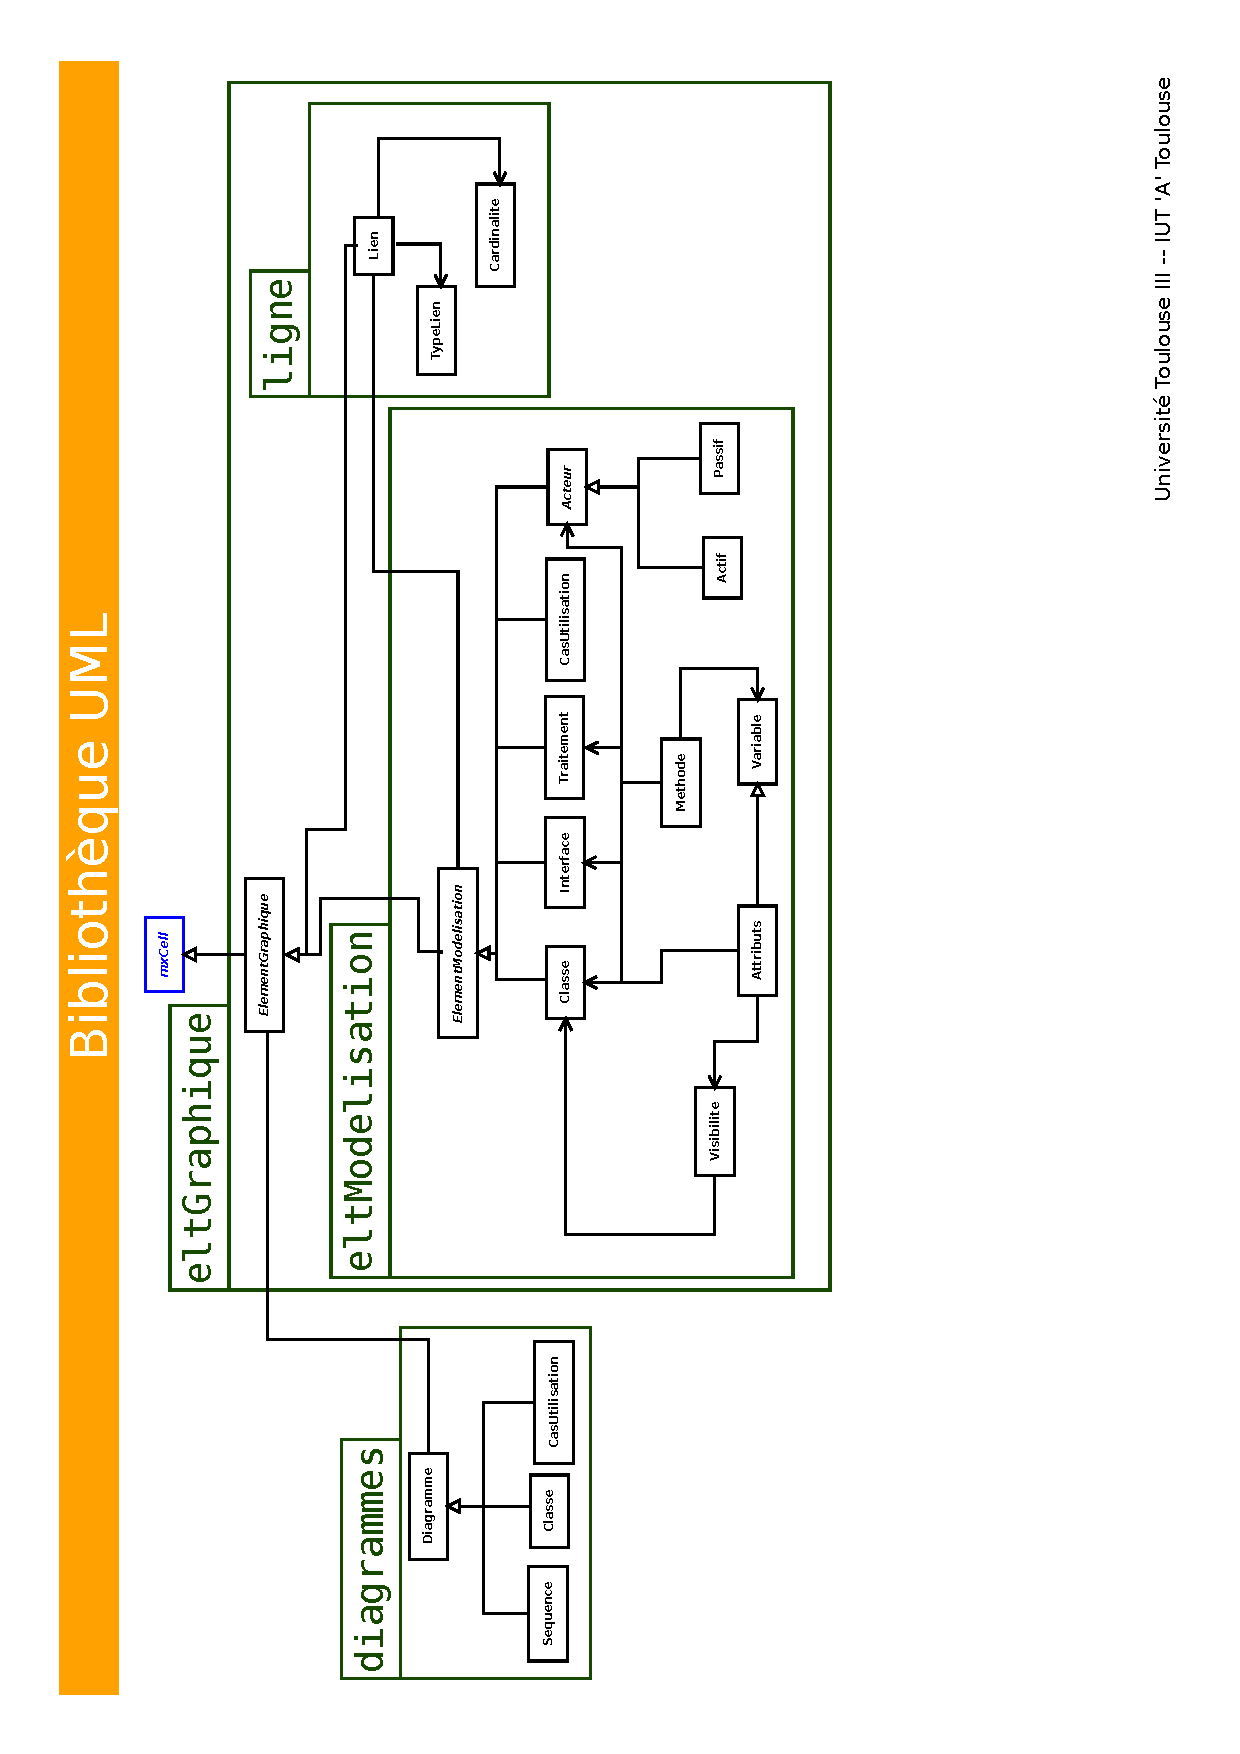
\includepdf{paquetageSansMethodes.pdf}
	\chapter{Diagramme de paquetages} \label{diagPaquetages}
	\nouveauChapitre
	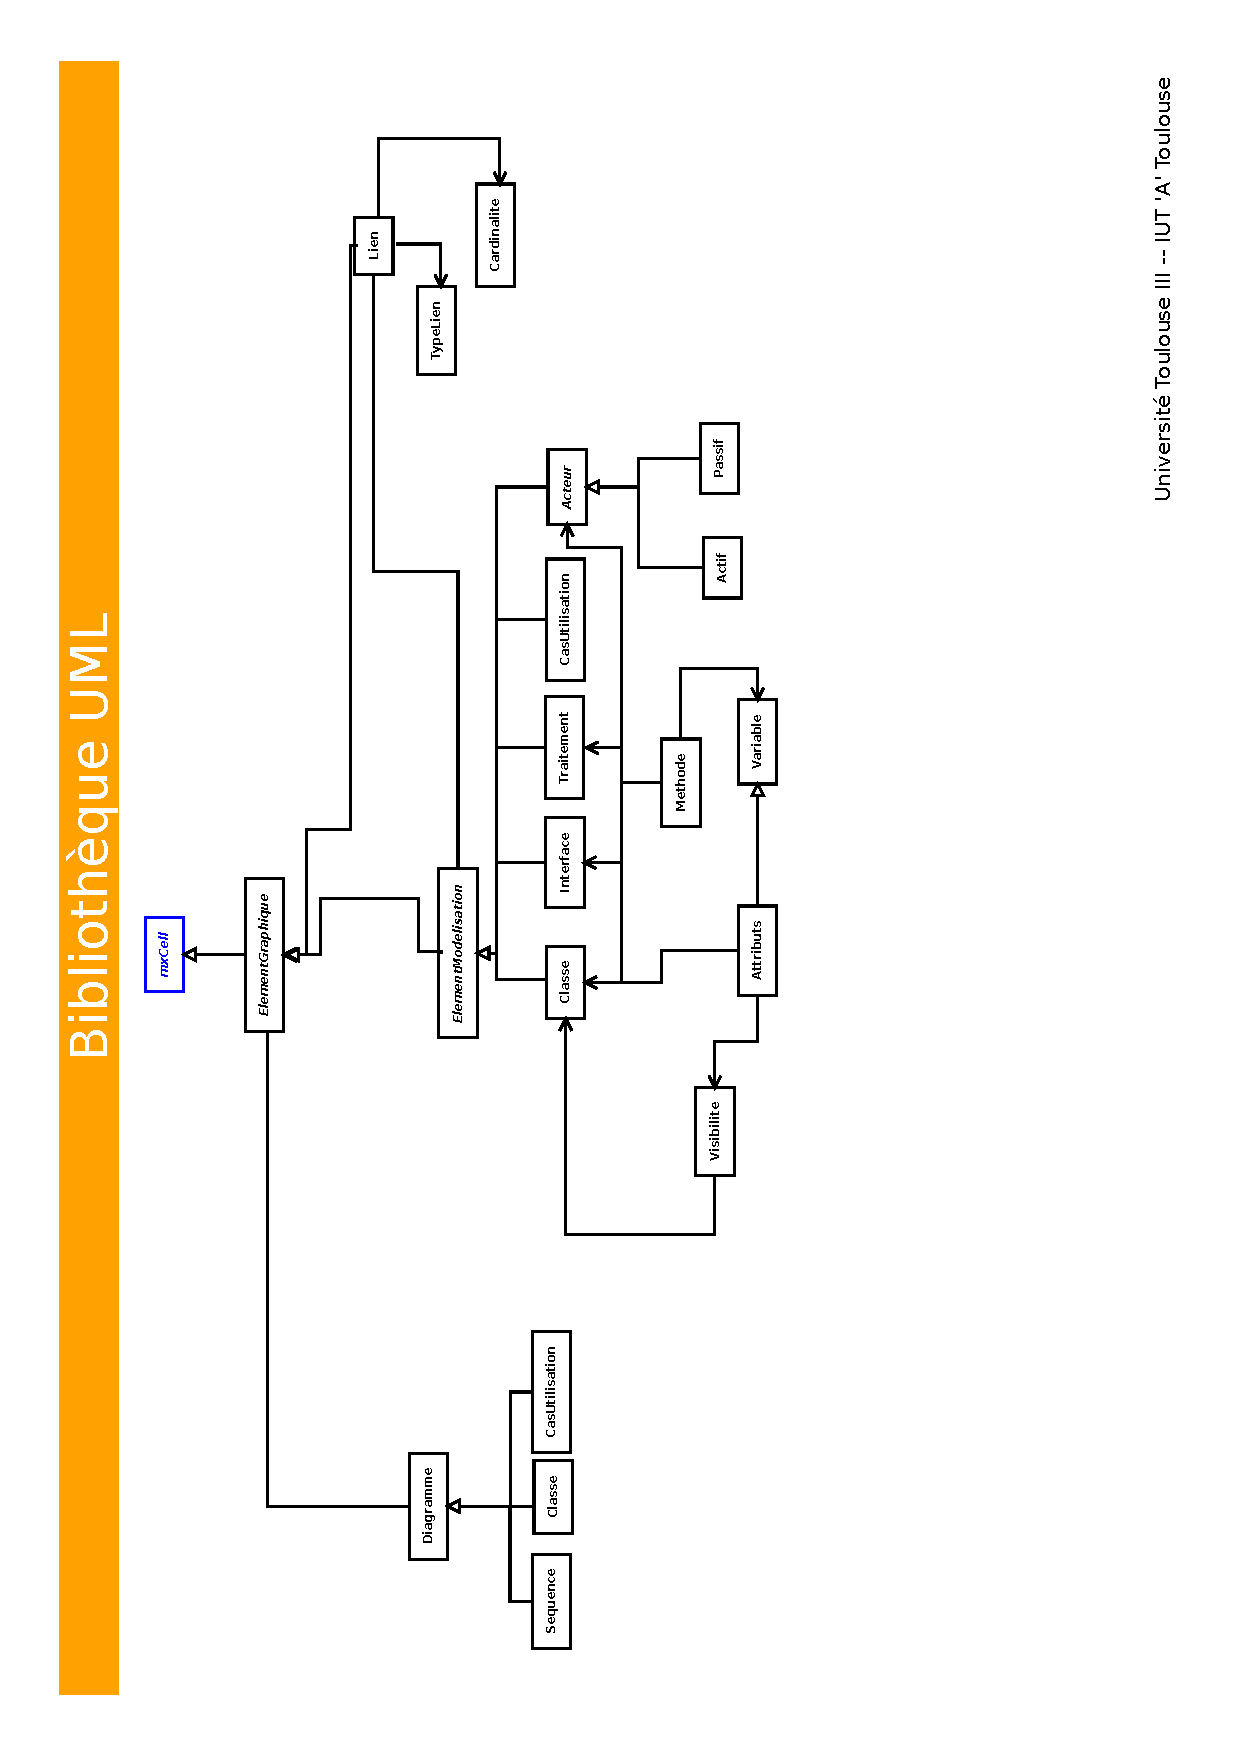
\includepdf{classeSansMethodes.pdf}
\end{document}

